
\chapter{First Appendix}

\section{Information Sheets}
\label{app:infoSheets}

\section{Consent Sheets}
\label{app:ConSheets}
- Probably don't need examples of each consent / information sheet from each studies. Probably just take the one I used for the media experiences project?

\section{Data management}
\label{app:DataManagement}
- Data Management PDF from the first case study

\section{Thematic Analysis Example}
\label{app:TA}
- Take this from NVivo - print out the codebook
\chapter{DemVR}
\section{Participants' final ideas}
\label{sec:EventIdeas}

\begin{figure}[htbp]
\begin{subfigure}[t]{0.3\textwidth}
    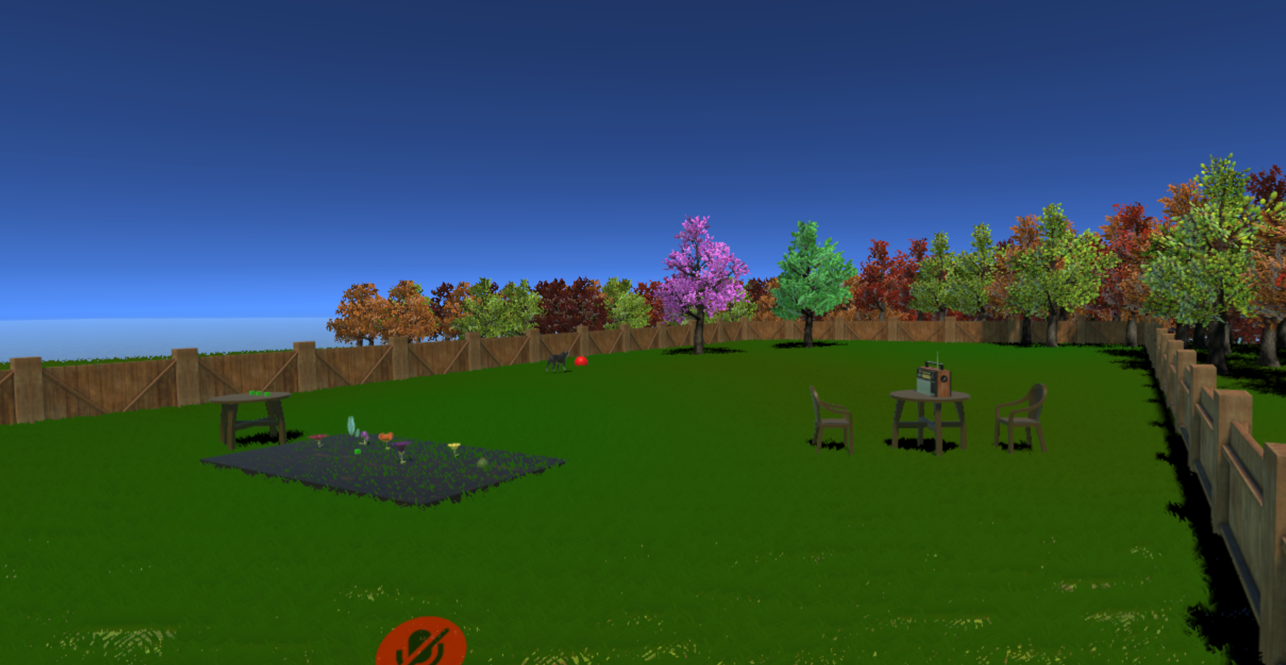
\includegraphics[width=\linewidth]{Images/DemVR/GardenLife.png}
\caption{Garden Life}
\label{fig:gardenLife}
\end{subfigure}\hfill
\begin{subfigure}[t]{0.3\textwidth}
  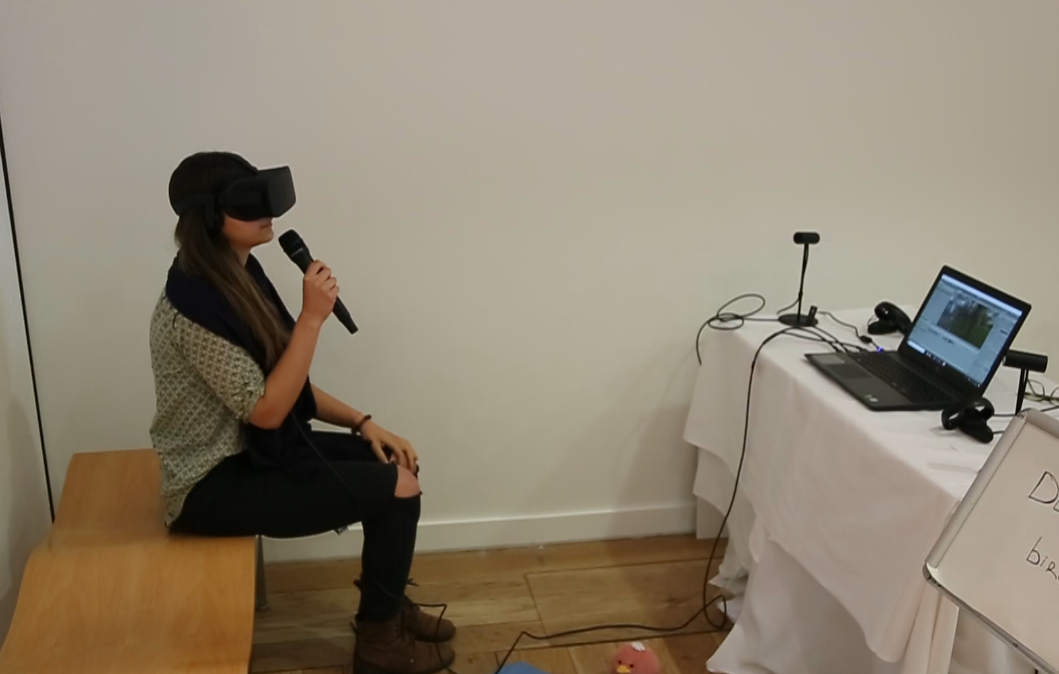
\includegraphics[width=\linewidth]{Images/DemVR/ChatterBench.png}
\caption{Chatter Bench}
\label{fig:ChatterBench}
\end{subfigure}\hfill
\begin{subfigure}[t]{0.3\textwidth}
    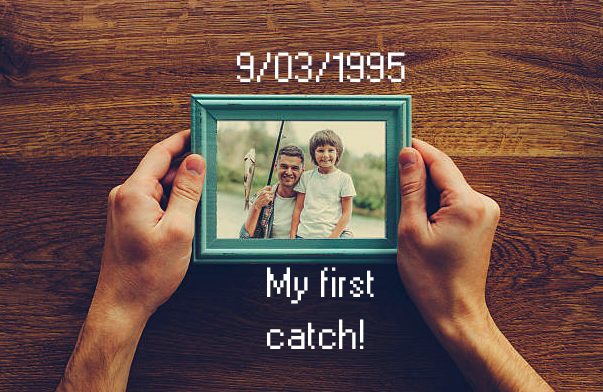
\includegraphics[width=\linewidth]{Images/DemVR/AugmentedWorld.png}
\caption{Augmented World}
\label{fig:AugmentedWorld}
\end{subfigure}

\begin{subfigure}[t]{0.3\textwidth}
    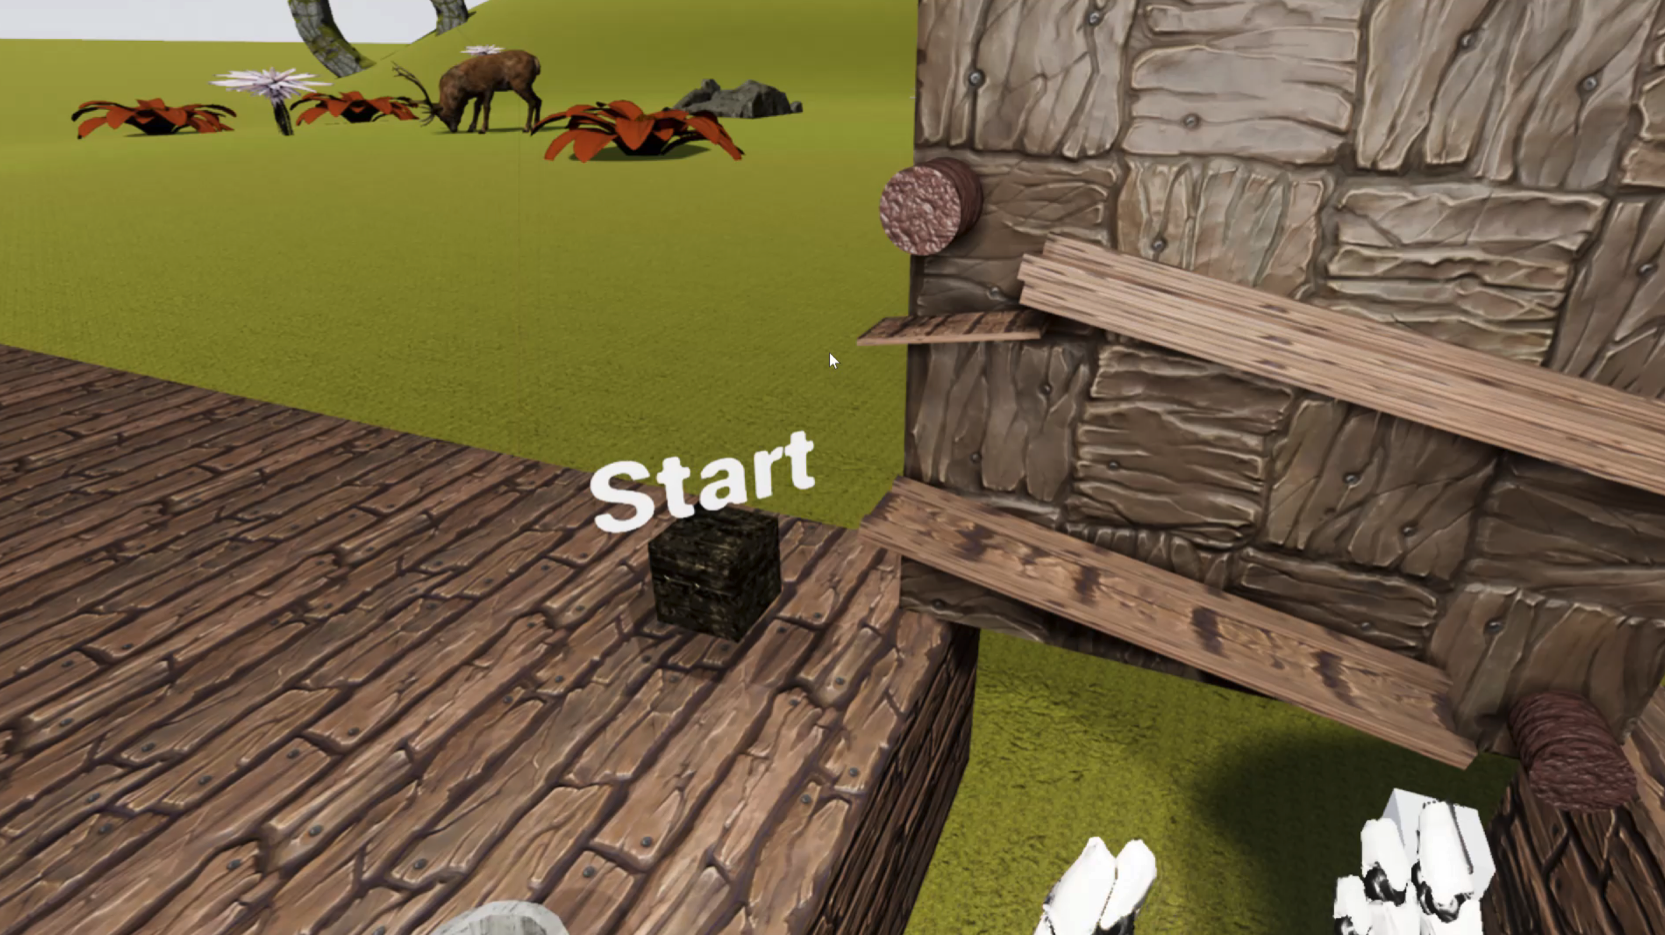
\includegraphics[width=\linewidth]{Images/DemVR/VRHallucinate.png}
\caption{VRHallucinate}
\label{fig:VRHallucinate}
\end{subfigure}\hfill
\begin{subfigure}[t]{0.3\textwidth}
    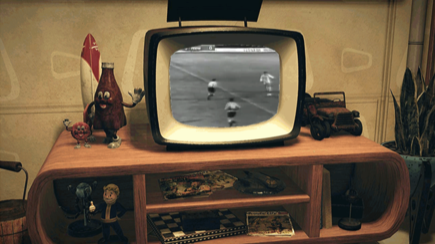
\includegraphics[width=\linewidth]{Images/DemVR/LookingVRBack.png}
\caption{Looking VR Back}
\label{fig:LookingVRBack}
\end{subfigure}\hfill
\begin{subfigure}[t]{0.3\textwidth}
    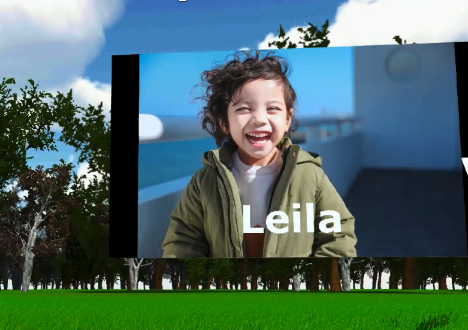
\includegraphics[width=\textwidth]{Images/DemVR/MindfulForest.png}
\caption{Mindful Forest}
\label{fig:MindfulForest}
\end{subfigure}

\begin{subfigure}[t]{0.3\textwidth}
    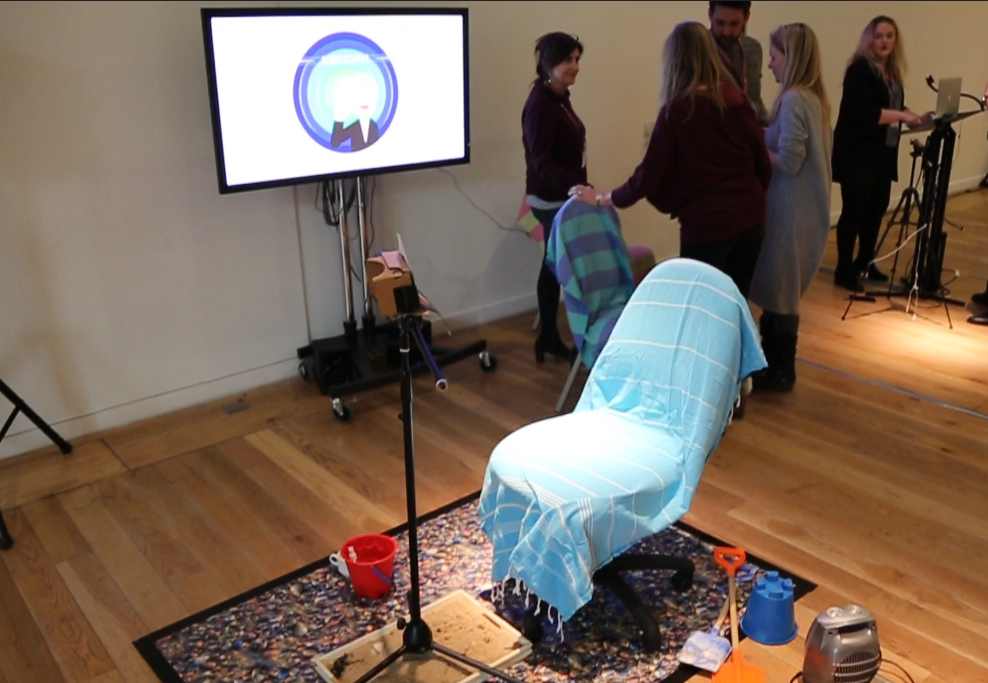
\includegraphics[width=\linewidth]{Images/DemVR/SensoryTides.png}
\caption{Sensory Tide}
\label{fig:SensoryTide}
\end{subfigure}\hfill
\begin{subfigure}[t]{0.3\textwidth}
    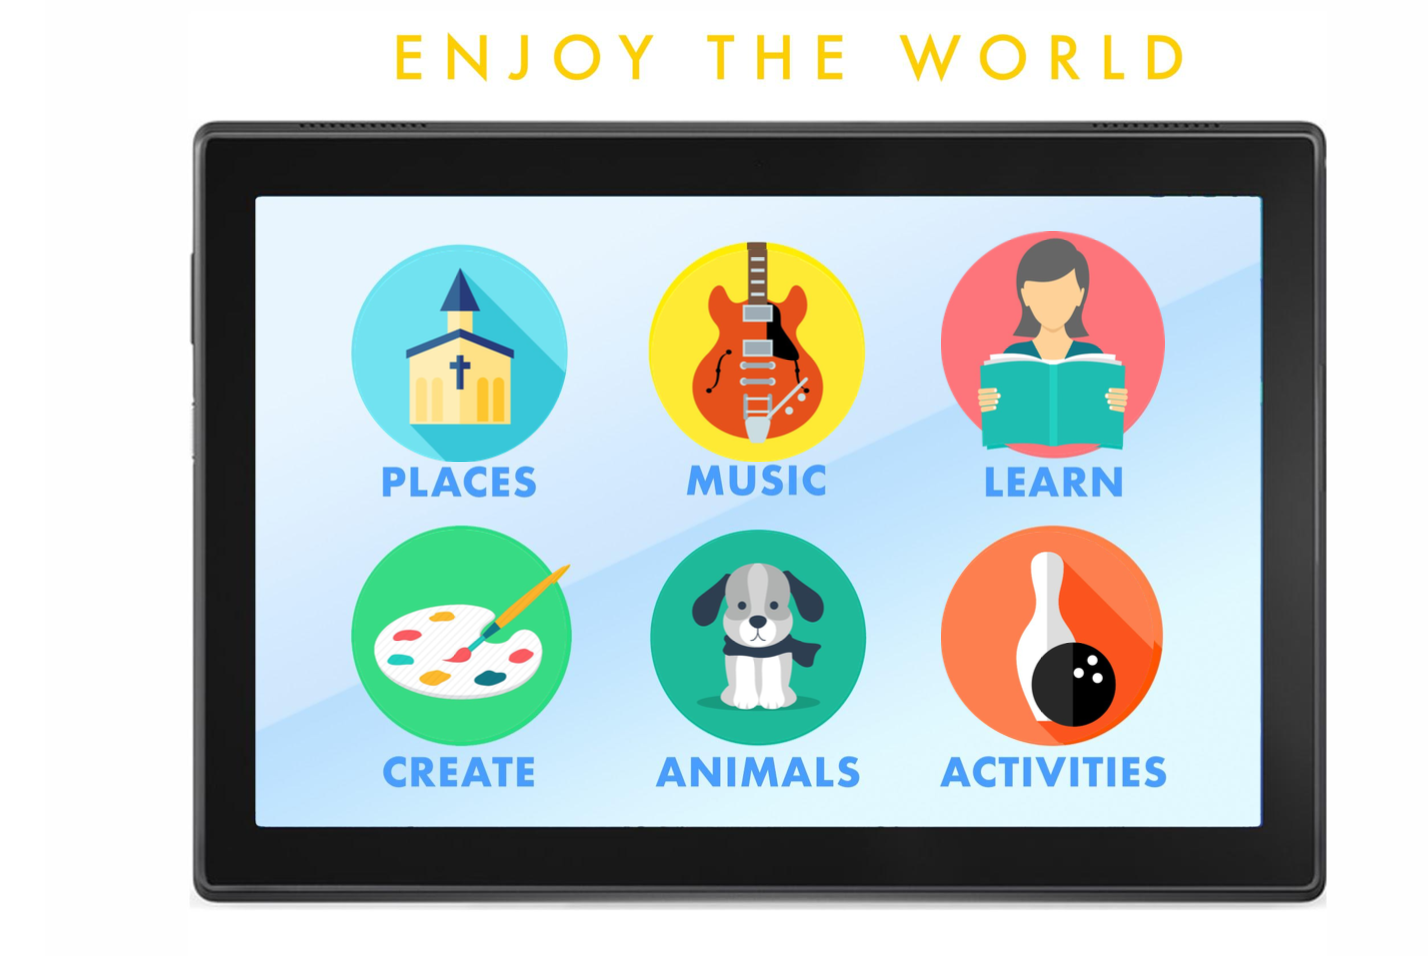
\includegraphics[width=\linewidth]{Images/DemVR/WorldShare.png}
\caption{WorldShare}
\label{fig:WorldShare}
\end{subfigure}\hfill
\begin{subfigure}[t]{0.3\textwidth}
    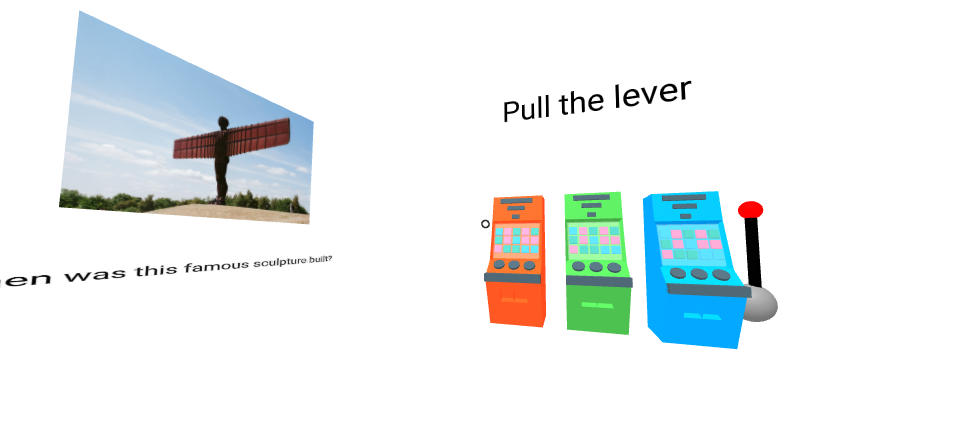
\includegraphics[width=\linewidth]{Images/DemVR/VRMotion.png}
\caption{VRMotion}
\label{fig:VRMotion}
\end{subfigure}
\caption{DemVR final prototype ideas}
\label{fig:DemVRFinalIdeas}
\end{figure}
From the final nine ideas, each team developed a prototype of their final idea alongside their ten minute presentation. In this subsection, I briefly breakdown each teams' proposed ideas and their final ideas:

\subsubsection{a. Garden Life (seven undergraduate computing students}
\label{sec:gardenLife}
\textbf{Proposed Idea:} Garden Life's proposed idea originated from Ideaboard where their idea would be to \textit{"create a journey through the story of your life using media that links memories with locations."}

\textbf{Final Idea:} In the teams' final idea, they created a VR garden and dog companion for those living in isolation without access to either in real life. The team had considered ways for sharing experiences by carers assisting the growth of a virtual garden through the extension of a tablet while the person living with dementia used VR. Furthermore, the team added multiplayer aspects to the experience allowing family and friends to virtually join the user in their own personalised garden with their virtual dog. 

\subsubsection{b. Chatter Bench (two designer / researchers) - Won 2nd Prize}
\label{sec:chatterbench}
\textbf{Proposed idea:} A chat-based VR experience that will consider the importance of sensitivity and aesthetic design. This idea was not developed on Ideaboard, but came from conversations between the two team members.

\textbf{Final Idea:} In teams' final idea, they developed a shared VR experience in Unity game engine where two users could 'sit' and talk on a virtual bench. Either the care partner, or person living with dementia could select from an array of different 360-degree environments where the two users could talk into a microphone and hear one another.

\subsubsection{c. Augmented World (six undergraduate computing students}
\label{sec:augmentedWorld}
\textbf{Proposed Idea:} A bespoke chronological AR timeline connected to experiences of the users past and family. The proposed idea was developed on Ideaboard by two of the six members who originally focused their idea on themes of reminiscence. 

\textbf{Final Idea:} An AR app that 'enhances' environmental objects to facilitate meaningful social interaction by connecting virtual objects to overlay on the real-life object. For example, a user can scan a picture of their family in the app which will then overlay virtual text or videos onto the picture.

\subsubsection{d. VRHallucinate (six members from developer, researcher, and UX backgrounds}
\label{sec:VRHallucinate}
\textbf{Proposed Idea:} As the team joined the event late and missed the pre-engagement phase, the team decided to develop a gamified experience to visualise hallucination-like effects to raise awareness of potential cognitive deficits that one may get with a diagnosis of dementia.

\textbf{Final Idea:} Similar to their proposed idea, they designed the hallucination game but targeted elements of ways to educate family, friends and the public surrounding the potential challenges of living with dementia.

\subsubsection{e. Looking VR Back (four members from marketing, development, biomedical backgrounds}
\label{sec:VRBack}

\textbf{Proposed Idea:} Using sounds, scents, and colours as a way to support reminiscence - this was proposed on Ideaboard by the same team.

\textbf{Final Idea:} Same idea but used a personalised example relating to Newcastle football game in 1969 as a way to take people living with dementia back to the particular experience through scents, sounds and 60-70's VR room aesthetic. 

\subsubsection{f. Mindful Forest (two undergraduate computing students}
\label{sec:mindfulForest}

\textbf{Proposed Idea:} A fantasy shared experience where families can add videos to trigger past memories. This idea was developed at the event as the team did not engage with Ideaboard.

\textbf{Final Idea:} A forest-like environment with gentle music and scenery. Families and friends can add videos to help with memory stimulation.

\subsubsection{g. Sensory Tide (six members from developer, researcher, and film backgrounds) - Won 1st Prize}
\label{sec:senosryTide}

\textbf{Proposed Idea:} The team combined several participants during the team formation, where multiple Ideaboard ideas came together. At the initial stage of developing their idea, the team had ideas of: replacing VR headsets with full-dome projections, themes of focusing on designing for the moment, as oppose to improving cognitive deficits, and designing reminiscence tools to increase Independence doing tasks.

\textbf{Final Idea:} The team developed an adapted version of a headset to resemble a beach telescope that was easily accessible. Additionally, the team created the VR beach experience to support multi-sensory needs for example, the user could smell seaweed in the room, a heated fan attached to the wall and sand under the feed of the user. 

\subsubsection{h. World Share (three filmmakers}
\label{sec:WorldShare}

\textbf{Proposed Idea:} Developed at the event, the team's initial idea was a tablet-based app to allow people living with dementia to 'travel' across the world and take part in tours and explore other scenic outdoor locations.

\textbf{Final Idea:} The final idea consisting of the following: a tablet that acts as a controller for interaction, and a headset to be used by the person living with dementia. The person with dementia would then request an event or a family recorded experience which the care partner would navigate to on the tablet and send the video/experience to the VR headset.

\subsubsection{i. VRMotion (for members from developer and researcher backgrounds)}
\label{VRMotion}
\textbf{Proposed Idea:} Influenced by their prior work in research, the team's initial idea was care home oriented where the VR experience would be a celebration of abilities of the individual instead of trying to bridge the abilities they have lost. 

\textbf{Final Idea:} Building from their proposed idea, they developed a shared virtual world where people with dementia can take part in group activities such as songs to sing along, guess the place, and solve the riddle - that was inspired by the work of Foley et al. \citep{foley_printer_2019}

\section{DemVR Event programme}
\label{app:DemVREvent}
Below, I provide the detailed event programme that I used for the advertisement and schedule material. In here you will find the event overview and the event schedule. 

\section{DemVR Recruitment Advertisement}
\label{app:DemVRRecruitment}
- the different advertisement we used / flyers / posters / website

\subsection{Event Overview}
\label{app:DemVR:Overview}
A big focus in dementia and technology research has been to tackle the cognitive deficits that often accompany the condition. Virtual reality has been used in the assessment and rehabilitation of cognitive processes in dementia since the 1990s, and more recently it's been used to deliver exergames. These developments are no doubt exciting - however, the potential for virtual reality as an expressive and creative medium to allow people with dementia to experience new, exciting, stimulating and potentially therapeutic environments, entirely separate from the stress of cognitive assessment, should also be addressed.

This event, organised by Newcastle University and held in central Newcastle, will provide an environment for innovative and creative ideas to emerge surrounding how we might create enriching shared experiences for people living with dementia. At the beginning of this two-day hackathon, we will help to `matchmake' participants and aid in the formation of multidisciplinary teams (ready-formed teams are also welcome!). Saturday morning will see the event introduced by keynotes from industry, research, and practice experts. Teams will be provided with creative material and qualitative data gathered from people living with dementia, as well as research from experts in the area of technology and dementia, in order to inspire them to create assets and environments that might enrich the shared experiences of those affected by the condition. After a solid 24 hours+ where participants are free to ideate, design, hack and make to their hearts' content, teams will have the opportunity to demonstrate, and present their reasoning behind their design choices to a team of expert judges in dementia care and research, who will award a monetary prize to the winning team.   

\textbf{First Prize: £1000}

\textbf{Second Prize: £500}



\subsection{Event schedule}
\label{app:DemVR:EventSchedule}
\begin{figure}[htp]
    \centering
    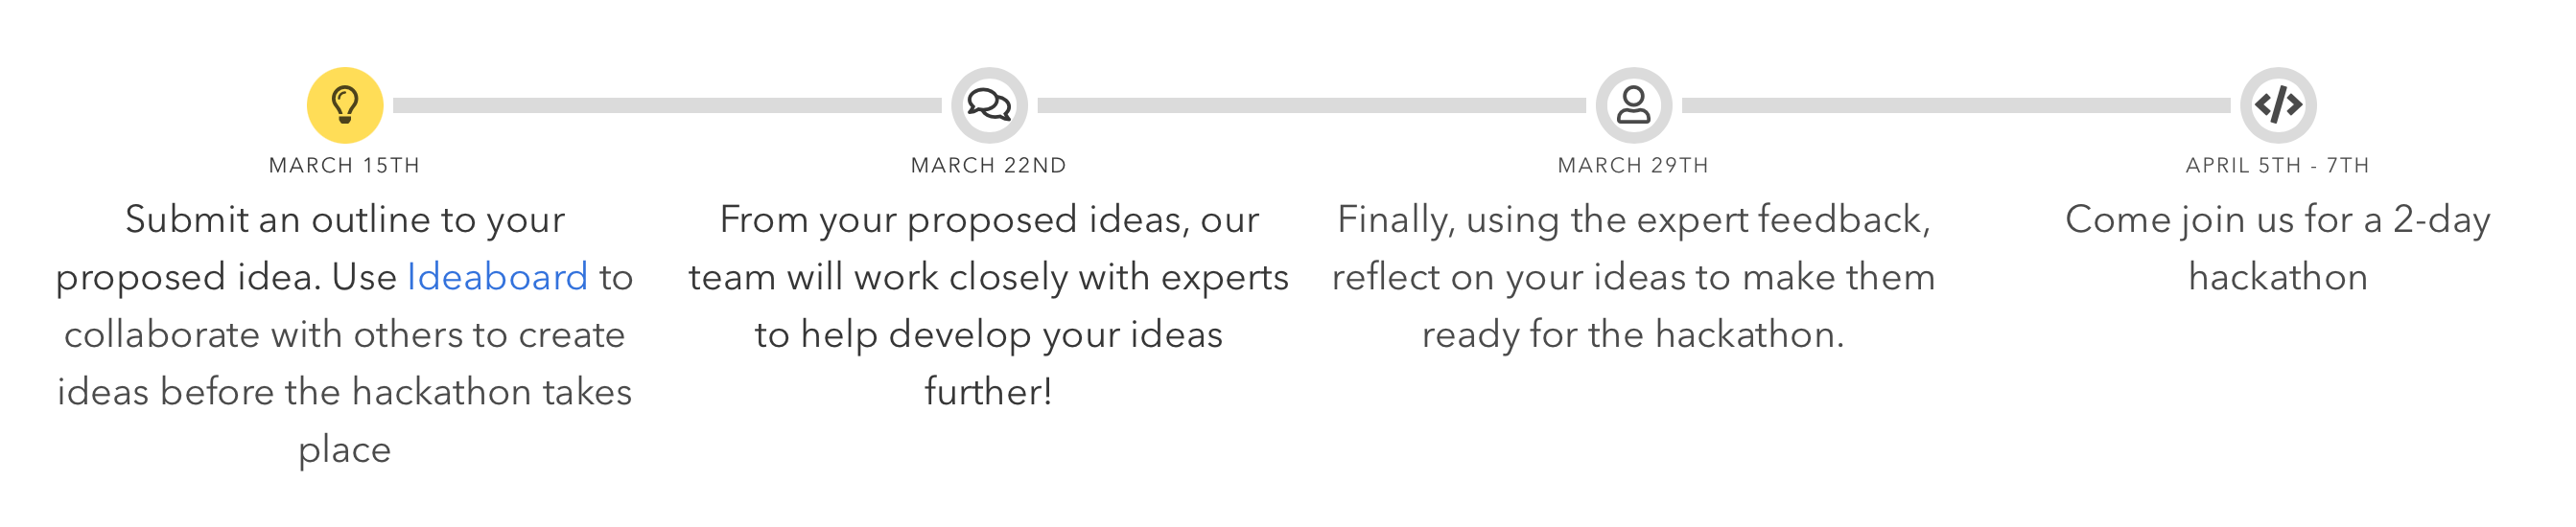
\includegraphics[width=0.8\linewidth]{Images/Appendix/DemVR appendix/Schedule.png}
    \caption{Schedule of DemVR}
    \label{fig:App:DemVRSchedule}
\end{figure}

% Please add the following required packages to your document preamble:
% \usepackage{graphicx}
\begin{table}[htbp]
\caption{DemVR two-day detailed schedule}
\label{tab:DemVR-Detailed schedule}
\resizebox{\columnwidth}{!}{%
\begin{tabular}{l|ll}
\textbf{\begin{tabular}[c]{@{}l@{}}Pre-hackathon\\ (In-person),\\ Friday, April 5, 2019\end{tabular}} &
  \begin{tabular}[c]{@{}l@{}}TEAM FORMATION\\ \\ Team formation will be held at Newcastle\\ \\ Pre-registration will be held on Friday before the hackathon starts to bring \\ participants together for team formation. We will also do an overview of the ideas \\ created on ideaboard. Feel free to choose one of these ideas or start from scratch \\ and create your own. Coming to the Friday event will help designers and \\ developers understand what is expected over the weekend and to get to know \\ everyone who is taking part in the hackathon.\\  \\ Recommended team size: 3-6\\ \\ 6pm: Meet and Greet / registration \\ 7pm: Team Formation \\ 8pm: Food / Drinks in town (at own cost)\end{tabular} &
   \\ \cline{1-2} \\
\textbf{\begin{tabular}[c]{@{}l@{}}Day 1\\ Hackathon,\\ Saturday, April 6, 2019\end{tabular}} &
  \begin{tabular}[c]{@{}l@{}}HACKATHON\\ The hackathon will begin Saturday morning with all teams formed \\ (any teams not organised, will be organised on the morning). The \\ day will start out with three keynote speakers talking about their \\ experiences about designing technology with people living with \\ dementia. Afterwards, teams will have free rein to work on their \\ designs for over 24 hours. \\ \\ INTRODUCTIONS \\ 8am - 9am: Breakfast \& registration (if you haven't registered on Friday) \\ 9am - 10am: Keynote Presentations \\ \\ HACKING STARTS \\ 10am – 11am: Start working on your idea\\ 10:30am – 11am: WhatsApp reflection period\\ 11am – 11:15am: tea, coffee, and biscuits\\ 11:15am – 12pm: Online Q\&A with Howard\\ 12pm – 1pm: WhatsApp reflection period\\ 1pm – 2pm: Lunch to be served\\ 2pm – 2:30pm: Pitch your idea to the room + Get feedback from Experts \\ 4:30pm - 5pm: Pitch Back \\ 6:30pm: Dinner\end{tabular} &
   \\ \cline{1-2} \\
\textbf{\begin{tabular}[c]{@{}l@{}}Day 2,\\ Judging,\\ Sunday, April 7, 2019\end{tabular}} &
  \begin{tabular}[c]{@{}l@{}}JUDGING\\ Sunday morning will give teams time to finalise their ideas and \\ set up for judging. Each team will present their idea and creations \\ to a panel of judges comprised of domain experts, designers. \\ Prizes will be awarded based on creativity, originality, and \\ project demonstration. \\  \\ 9am - 10am: Breakfast \\ 9am - 10am: WhatsApp reflection period\\ 11am – 11:30am: Tea, coffee, and biscuits\\ 12pm – 1pm: Lunch to be served\\ 1pm – 2pm: WhatsApp reflection period \\ 2:15pm – 4pm: Team presentations\\ 4pm – 4:20pm: Judges scoring \& WhatsApp reflection period*\\ 4:20pm 5pm: Awards and closing\end{tabular} &
  
\end{tabular}%
}
\end{table}

\chapter{Appendix C}

\section{Ethics Semi-structured interview}
\label{app:EthicInterview}
The following questions were used for the 22 interviews with HCI researchers seen in chapter \ref{EthicsChapter}.

\begin{enumerate}

   \item \textbf{What work have you done in a dementia context?}
\begin{enumerate}
        \item Can you elaborate on our expertise and experience?
\end{enumerate}

    \item \textbf{What do you think about the role of the individual researcher vs. the institutional responses to protecting researchers}
    \begin{enumerate}
        \item Can you tell me a bit about your interactions with ethical review processes at your institution?
        \item Do you think that they are effective at protecting participants? Researchers?
        \item How do you think they change when you talk about technology as being a part of your work?
    \end{enumerate}

    \item \textbf{How do you think implementing technology into technology has added to the ethical complexities of working with people living with dementia?}
    \begin{enumerate}
        \item Do you think that seeking to innovate technologically has made working with people with dementia more ethically complex? If so, how?
        \item How do you think such work is perceived by the media? The larger research community?
        \item Do you think people with dementia and their carers/families want technology in their lives?
    \end{enumerate}

    \item \textbf{Have you felt a power imbalance of sorts between you as the researcher or significant role changes between the carer and the person with dementia?}
    \begin{enumerate}
        \item Can you tell me a bit about the sorts of relationships you’ve had in dementia contexts?
        \item (if there are many) What do you feel was the most interesting or striking relationship?
        \item In particular, I’m interested in a sense of power balance or imbalance, or instances where your role changed.
    \end{enumerate}

    \item \textbf{Have you had instances where you’ve become part of a community/friends with your participants? Do you feel there is a line? Are the steps you’d suggest to other researchers to follow or have in the back of their heads?}
    \begin{enumerate}
        \item Have you had instances where you’ve become part of a community or friends with your participants?
        \item Do you feel there is a line that should or shouldn’t be crossed?
        \item Are the steps you’d suggest to other researchers to follow or have in the back of their heads if this is something that’s happening for them?
    \end{enumerate}

    \item \textbf{How can we make sure our efforts have longevity?}
    \begin{enumerate}
        \item Do you feel like your research, or HCI research into dementia in general, has longevity?
        \item What are some ways we can extend our longevity?
        \item Are there instances where longevity isn’t as important as we might think?
    \end{enumerate}

    \item \textbf{Questioning reliability of technology vs short and fast iteration of technology}
    \begin{enumerate}
        \item How highly do you value the reliability of the technologies you create?
        \item Do you feel like agile design environments or processes are suitable to the creation of technologies for people with dementia?
        \item Can you describe some of the design processes you’ve undertaken with people with dementia in the past, from a methods point of view?
    \end{enumerate}

    \item D\textbf{esigning for an exit strategy. It needs to be more than just a debrief document.}
    \begin{enumerate}
        \item Negotiating a process of leaving can be difficult when you’ve come to form attachments to your participants. Can you tell me a bit about how you’ve left research contexts in the past?
        \item What about leaving technologies or designs behind? What sort of responsibilities do we have then?
    \end{enumerate}

    \item \textbf{Anonymisation is a key premise of how we conduct ethical research to protect the privacy and integrity of those we’re working with. While we typically default to this, do you think thats a good idea? Are we hindering acknowledgment of those we’re working with and not crediting their creative and intellectual work.}
    \begin{enumerate}
        \item How do you feel about anonymisation in design research with dementia?
        \item Is it always a good thing, or is it more ethical to identify participants’ achievements and labour?
        \item What would an updated best practice look like here?
    \end{enumerate}

    \item \textbf{How useful are examination boards? How much do they know about the research they are overseeing and do they see the clear benefits of the research we’re doing?}
    \begin{enumerate}
        \item Can you tell me about your experiences with ethical review boards?
        \item How much do you feel they know about the research they are passing judgement on?
        \item Do they always see the benefits of our research?
        \item When we are working in an ethically dynamic environment to what extent are ethical review boards aware of the changing environment or restrict ground breaking research in this area?
    \end{enumerate}
 
    \item \textbf{At what point should we publish? Should we place quality over quantity in publications? How can we challenge the problems of expectations from participants from previous work?}
\end{enumerate}

\section{Affinity Diagramming}
\label{app:AD}
- Miro images of the affinity diagramming in the toolkit paper

\section{Workshop materials}
\label{app:ToolkitMaterials}
- Pull in images of the different workout materials from the workshops I made